\documentclass[10pt,a4paper]{article}
\usepackage[utf8]{inputenc}
\usepackage[T1]{fontenc}
\usepackage{amsmath,amssymb,amsthm,mathtools}
\usepackage{geometry}
\geometry{margin=2.1cm}
\usepackage{booktabs}
\usepackage{xcolor}
\usepackage{enumitem}
\usepackage{array}
\usepackage{lmodern}
\usepackage{microtype}
\usepackage{tikz}
\usepackage{hyperref}
\hypersetup{
    colorlinks=true,
    linkcolor=blue!70!black,
    citecolor=red!70!black,
    urlcolor=blue!70!black,
    pdftitle={Cauchy-Schwarz Lower Bounds, Dirichlet Anchoring, Two-Dimensional Abel Telescoping, and the Pure Plaque Vanishing Criterion},
    pdfauthor={Qamar Munawer}
}

\newtheorem{theorem}{Theorem}[section]
\newtheorem{lemma}[theorem]{Lemma}
\newtheorem{corollary}[theorem]{Corollary}
\theoremstyle{definition}
\newtheorem{definition}[theorem]{Definition}
\newtheorem{remark}[theorem]{Remark}

\title{\textbf{Pure Plaque Cauchy--Schwarz Bounds, Dirichlet Anchoring ($c_1 = -1$),\\
Two-Dimensional Abel Telescoping, and the Plaque Vanishing Criterion}}

\author{\textbf{Qamar Munawer}\\[0.2em]
\small Brandenburg University of Technology Cottbus--Senftenberg, Cottbus, Germany}

\date{November 18, 2026}

\begin{document}
\linespread{1.11}\selectfont
\emergencystretch=2.5em

\maketitle

\begin{abstract}
Under the standing epistemic invariant \texttt{NO\_RH\_PROOF = TRUE}, this paper attacks the finite-dimensional cotangent frontier left open by the boundary-plus-plaque split on the B\'aez--Duarte affine manifold. Ten self-contained modular Lean~4.35 units in Wave~8 (\texttt{UpstreamPR\_8A}--\texttt{8J}, bringing the standalone archive to fifty-three linter-verified modules with zero \texttt{sorry}s, zero linter errors across fifteen checks, and standard axioms only) formalize the analytical, algebraic, exact-certificate, universal superdiagonal, and unit-partition pillars of the pure plaque program. First, applying the scale-invariant cotangent Cauchy--Schwarz inequality along tangent shifts isolates an explicit quadratic lower bound on the pure plaque form and yields a universal $-h_1^2/4$ floor. Second, imposing the Dirichlet pole lock $c_1 = -1$ ($h_1 = 1$) cancels the leading linear drive against the anchor boundary shift, guaranteeing non-negativity of the pure plaque form whenever the normalized linear cotangent drive is at least $1$, and identifying the unit-drive Dirichlet plaque energy identically with the squared $L^2(0,1)$ Nyman--Beurling residual. Third, a two-dimensional discrete Abel telescoping theorem compresses the four-point plaque double sum over $[1,N-2]^2$ into a boundary-subtracted unweighted Vasyunin kernel bilinear form on $[3,N]^2$. Fourth, universal shift periodicity $V(a, a+r) = V(a, r)$ and reflection $V(a, a-r) = -V(a, r)$ prove the all-$m$ superdiagonal orthogonality theorem $\widetilde{G}_{m, m+1} = 0$ for every $m \ge 1$, exact $N=6$ block-trace radical cancellation $\widetilde{G}_{33} + \widetilde{G}_{44} = \pi(4/\sqrt{3} - 1)$, and the unit-partition homogeneous kernel reduction $1 - S_{\mathrm{cot}}(c,N) = \sum_{a,b} \alpha_a\alpha_b \mathcal{M}_{ab} \ge 0$ with $\mathcal{M}_{12} = 1 - \pi/2 < 0$, $\mathcal{M}_{11}+\mathcal{M}_{22}=2$, and $\mathcal{M}_{33}+\mathcal{M}_{44}=2+\frac{2\pi}{3\sqrt{3}}$. Eighty-digit \texttt{mpmath} experiments from $N=4$ to $N=64$ verify all discrete identities and closed-form $N=4,5,6$ Gram laws to within $2.5 \times 10^{-85}$.
\end{abstract}

\noindent\textbf{Keywords:} B\'aez--Duarte criterion, pure plaque kernel, Dirichlet anchoring, 2D Abel telescoping, unit-partition duality, Lean~4, \texttt{NO\_RH\_PROOF = TRUE}.

\section{Epistemic Scope and Wave 8 Lean 4 Architecture}

All theorems reported below adhere strictly to \texttt{NO\_RH\_PROOF = TRUE}: they establish unconditional algebraic identities, quadratic inequalities, discrete telescoping reductions, and conditional $L^2(0,1)$ criteria for the Riemann Hypothesis without claiming an unconditional proof of RH. Wave~8's standalone modular units (\texttt{UpstreamPR\_8A}--\texttt{8J}) compile cleanly under \texttt{leanprover--lean4---v4.35.0} with \texttt{0} errors across all $15$ Mathlib/Batteries linters (\texttt{\#lint}) and depend strictly on standard axioms \texttt{[propext, Classical.choice, Quot.sound]} within the $53$-module verified archive:
\begin{enumerate}[leftmargin=1.8em,itemsep=1pt]
\item \texttt{BaezDuartePlaqueCauchySchwarz.lean} (\texttt{PR-8A}, $144$ lines): defines \texttt{dipolePlaqueForm}, proves shift invariance \texttt{dipolePlaqueForm\_\allowbreak sub\_cBaseAnchor\_eq}, derives \texttt{sq\_linearCotDrive\_\allowbreak sub\_le\_dipolePlaqueForm}, proves the universal $-h_1^2/4$ plaque floor, and establishes the unit-drive lower bound $1 - h_1 \le \mathcal{P}_N(h)$.
\item \texttt{BaezDuarte\allowbreak DirichletAnchoredPlaque.lean} (\texttt{PR-8B}, $147$ lines): defines \texttt{IsDirichletAnchored} ($D_1 = 0$, $D_0 = 2$, $c_1 = -1$) and the explicit $3$-term anchor \texttt{cDirichletAnchor} $= (-1, 0, 3, 0, \dots) = c_{\mathrm{base}} + \psi_1$, proves unconditional plaque positivity for $\pi L_{\mathrm{cot}}(h,N) \ge 1$, the universal $-1/4$ floor, and \texttt{unit\_drive\_\allowbreak dirichlet\_plaque\_eq\_l2\_dist}.
\item \texttt{BaezDuartePlaqueTelescoping.lean} (\texttt{PR-8C}, $168$ lines): proves \texttt{unweightedKCot\_\allowbreak two\_two\_eq\_zero}, the exact kernel rectangle telescoping identity \texttt{sum\_Icc\_\allowbreak dipolePlaqueEntry\_eq}, and \texttt{dipolePlaqueForm\_\allowbreak sub\_cBaseAnchor\_\allowbreak eq\_telescoped\_kernel}.
\item \texttt{BaezDuarte\allowbreak PurePlaqueRHCriterion.lean} (\texttt{PR-8D}, $239$ lines): defines \texttt{PurePlaque\allowbreak VanishingCriterion} and \texttt{TelescopedPlaque\allowbreak VanishingCriterion}, proves their equivalence, formalizes the off-line zero floor \texttt{purePlaque\_\allowbreak floor\_of\_zeta\_zero}, and proves \texttt{riemannHypothesis\_\allowbreak of\_purePlaque\_vanishing} assuming \texttt{TitchmarshMellinProperty}.
\item \texttt{BaezDuarteDirichletOptFour.lean} (\texttt{PR-8E}, $162$ lines): defines \texttt{cDirichletOptFour} at $\alpha_1 = \tfrac{1}{2} + \tfrac{1}{3\sqrt{3}}$, $\alpha_2 = \tfrac{1}{2} - \tfrac{1}{3\sqrt{3}}$, proves exact radical cancellation $S_{\mathrm{cot}}(c_{\mathrm{dir}}^{(4)}, 4) = \tfrac{31}{108}\pi$, and proves global optimality over all Dirichlet-anchored vectors on $\mathcal{A}_4$.
\item \texttt{BaezDuarteDipoleGramFive.lean} (\texttt{PR-8F}, $172$ lines; \texttt{UpstreamPR\_8F\_\allowbreak DipoleGramFiveCert.lean}): formalizes exact $(\mathbb{Z}/5\mathbb{Z})^\times$ reciprocity vanishing \texttt{dipoleGramEntry\_\allowbreak two\_three\_eq\_zero} and closed-form $N=5$ evaluations \texttt{dipoleGramEntry\_\allowbreak one\_three\_eq}, \texttt{dipoleGramEntry\_\allowbreak three\_three\_eq}, and \texttt{dipolePlaqueEntry\_\allowbreak two\_three\_eq}.
\item \texttt{BaezDuarteCotangentSix.lean} (\texttt{PR-8G}, $209$ lines; \texttt{UpstreamPR\_8G\_\allowbreak CotangentSixReciprocity.lean}): proves exact $a=6$ Vasyunin sums in $\mathbb{Q}(\sqrt{3})$, \texttt{deltaCot\_six\_eq} ($\tfrac{5}{3\sqrt{3}}$), divisibility orthogonality \texttt{unweightedKCot\_\allowbreak three\_six\_eq\_zero}, horizontal telescoping \texttt{dipoleGramEntry\_\allowbreak add\_succ\_right}, \texttt{dipoleGramEntry\_\allowbreak one\_four\_eq}, and decoupling \texttt{dipoleGramEntry\_\allowbreak two\_four\_eq\_zero}.
\item {\sloppy\texttt{Baez\allowbreak Duarte\allowbreak Superdiagonal\allowbreak Orthogonal\allowbreak Triple.lean} (\texttt{PR-8J}, $235$ lines; \texttt{UpstreamPR\_\allowbreak 8J\_\allowbreak Superdiagonal\allowbreak And\allowbreak Orthogonal\allowbreak Triple.lean}, extending \texttt{8H}--\texttt{8I}): proves \texttt{dipoleGramEntry\_\allowbreak self\_\allowbreak succ\_\allowbreak eq\_\allowbreak zero} ($\forall m \ge 1,\; \widetilde{G}_{m,m+1}=0$), \texttt{dipolePlaqueEntry\_\allowbreak self\_\allowbreak succ\_\allowbreak eq}, the orthogonal triple theorem \texttt{dipoleGramEntry\_\allowbreak orthogonal\_\allowbreak triple\_\allowbreak two\_\allowbreak three\_\allowbreak four} on $\{v^{(2)},v^{(3)},v^{(4)}\}$ and 3-mode Pythagorean energy law \texttt{QCot\_\allowbreak span\_\allowbreak two\_\allowbreak three\_\allowbreak four\_\allowbreak eq\_\allowbreak sum\_\allowbreak sq}, $N=6$ block trace \texttt{dipoleGramEntry\_\allowbreak three\_\allowbreak three\_\allowbreak add\_\allowbreak four\_\allowbreak four\_\allowbreak eq}, \texttt{isDirichlet\allowbreak Anchored\_\allowbreak unit\_\allowbreak partition}, the homogeneous kernel \texttt{unitDefectEntry}, trace laws ($2$ and $2 + 2\pi/(3\sqrt{3})$), and \texttt{one\_\allowbreak sub\_\allowbreak SCot\_\allowbreak eq\_\allowbreak sum\_\allowbreak unitDefectEntry\_\allowbreak of\_\allowbreak isDirichlet\allowbreak Anchored}.\par}
\end{enumerate}

\section{Pure Plaque Cauchy--Schwarz Inequality and Dirichlet Anchoring}

Let $\mathcal{A}_N = \{c : \mathbb{N} \to \mathbb{R} \mid D_1(c,N) = 0 \land D_0(c,N) = 2\}$ and let $\mathcal{A}_N^0 = \{h \mid D_1(h,N) = 0 \land D_0(h,N) = 0\}$ denote its tangent subspace anchored at $c_{\mathrm{base}} = (-2, 4, 0, \dots)$. Recall from \texttt{PR-7C} the unweighted Vasyunin kernel $K(j,k) = jk \, g_{j,k}^{(\mathrm{cot})}$ and the pure $4$-point plaque kernel $P(a,b) = K(a+1,b+1) - K(a+1,b+2) - K(a+2,b+1) + K(a+2,b+2)$. In cumulative suffix dipole coordinates $\eta_a = \sum_{j=a+2}^N h_j / j$ ($1 \le a \le N-2$), the \emph{total pure plaque quadratic form} is
\[
\mathcal{P}_N(h) := \sum_{a=1}^{N-2}\sum_{b=1}^{N-2} \eta_a(h) \eta_b(h) P(a,b),
\qquad
\text{satisfying } \mathcal{P}_N(c - c_{\mathrm{base}}) = \mathcal{P}_N(c).
\]

\begin{theorem}[Pure Plaque Cauchy--Schwarz Lower Bounds, \texttt{PR-8A}]\label{thm:plaque_cs}
For every $N \ge 2$ and every tangent vector $h \in \mathcal{A}_N^0$:
\begin{enumerate}[leftmargin=1.8em,itemsep=2pt]
\item Combining $Q_{\mathrm{cot}}(h,N) = \pi h_1 L_{\mathrm{cot}}(h,N) + \mathcal{P}_N(h)$ with $(\pi L_{\mathrm{cot}}(h,N))^2 \le Q_{\mathrm{cot}}(h,N)$ yields
\begin{equation}\label{eq:plaque_cs}
\bigl(\pi L_{\mathrm{cot}}(h,N)\bigr)^2 - \pi h_1 L_{\mathrm{cot}}(h,N) \le \mathcal{P}_N(h).
\end{equation}
\item Completing the square in~\eqref{eq:plaque_cs} gives $(\pi L_{\mathrm{cot}}(h,N) - h_1/2)^2 - h_1^2/4 \le \mathcal{P}_N(h)$, hence universally $-h_1^2 / 4 \le \mathcal{P}_N(h)$.
\item Under the unit-drive normalization $\pi L_{\mathrm{cot}}(h,N) = 1$, inequality~\eqref{eq:plaque_cs} reduces to $1 - h_1 \le \mathcal{P}_N(h)$.
\end{enumerate}
\end{theorem}

The structural role of the Dirichlet pole condition $c_1 = -1$ ($h_1 = c_1 - c_{\mathrm{base},1} = 1$) now becomes immediate: on the $1$-codimensional affine slice $\mathcal{A}_N^{\mathrm{dir}} := \{c \in \mathcal{A}_N \mid c_1 = -1\}$, the $3$-term anchor $c_{\mathrm{dir}} = (-1, 0, 3, 0, \dots) = c_{\mathrm{base}} + \psi_1$ witnesses non-emptiness for all $N \ge 3$ (\texttt{cDirichletAnchor\_isDirichletAnchored}), while $\sum_{m=1}^{N-2} \eta_m = h_1 = 1$.

\begin{theorem}[Dirichlet-Anchored Plaque Positivity and Exact $L^2$ Energy Law, \texttt{PR-8B}]\label{thm:dirichlet}
Let $N \ge 2$, $c \in \mathcal{A}_N^{\mathrm{dir}}$ ($c_1 = -1$), and $h = c - c_{\mathrm{base}} \in \mathcal{A}_N^0$ ($h_1 = 1$). Then:
\begin{enumerate}[leftmargin=1.8em,itemsep=2pt]
\item Unconditionally, $-\tfrac{1}{4} \le \mathcal{P}_N(h)$ and $\bigl(\pi L_{\mathrm{cot}}(h,N)\bigr)^2 - \pi L_{\mathrm{cot}}(h,N) \le \mathcal{P}_N(h)$.
\item Whenever $1 \le \pi L_{\mathrm{cot}}(h,N)$, the pure plaque quadratic form is guaranteed non-negative: $\mathcal{P}_N(h) \ge 0$.
\item Along the full Dirichlet slice, $\int_0^1 \bigl(1 - \sum_{k=1}^N c_k \{1/(kx)\}\bigr)^2 dx = 1 - \pi L_{\mathrm{cot}}(h,N) + \mathcal{P}_N(h)$.
\item Restricting further to the unit-drive slice $\pi L_{\mathrm{cot}}(h,N) = 1$ cancels the constant and linear terms identically, isolating the $L^2(0,1)$ residual directly as the pure plaque form:
\begin{equation}\label{eq:unit_dir_energy}
\mathcal{P}_N(h) = \int_0^1 \left(1 - \sum_{k=1}^N c_k \left\{\frac{1}{kx}\right\}\right)^{\!2} dx \ge 0.
\end{equation}
\end{enumerate}
\end{theorem}

\section{Two-Dimensional Abel Telescoping and the Plaque RH Criterion}

Equation~\eqref{eq:unit_dir_energy} compresses the Nyman--Beurling approximation problem into driving $\mathcal{P}_N(c - c_{\mathrm{base}}) \to 0$ on the doubly constrained unit-drive Dirichlet slice $\{c \in \mathcal{A}_N \mid c_1 = -1,\, \pi L_{\mathrm{cot}}(c - c_{\mathrm{base}}, N) = 1\}$. Two-dimensional summation by parts translates this cumulative plaque form directly back into the physical vector $c_3, \dots, c_N$.

\begin{theorem}[2D Discrete Abel Telescoping Reduction, \texttt{PR-8C}]\label{thm:telescoping}
Using $V(2,b) = 0$ ($\cot(\pi/2) = 0$), the boundary node satisfies $K(2,2) = 0$ (\texttt{unweightedKCot\_two\_two\_eq\_zero}). Consequently, for every $j,k \ge 3$,
\begin{equation}\label{eq:kernel_tel}
\sum_{a=1}^{j-2}\sum_{b=1}^{k-2} P(a,b) = K(j,k) - K(j,2) - K(2,k),
\end{equation}
and for any vector $c \in \mathcal{A}_N$ with $h = c - c_{\mathrm{base}}$ (so $h_j = c_j$ for all $j \ge 3$),
\begin{equation}\label{eq:form_tel}
\mathcal{P}_N(h) = \sum_{j=3}^N \sum_{k=3}^N \frac{c_j c_k}{jk} \bigl(K(j,k) - K(j,2) - K(2,k)\bigr).
\end{equation}
\end{theorem}

Combining Theorem~\ref{thm:dirichlet}, Theorem~\ref{thm:telescoping}, the Mellin energy identity $\int_0^1 x^{2\sigma-2} dx = (2\sigma-1)^{-1}$ (\texttt{PR-7A}), and Titchmarsh's Mellin fractional-part formula \texttt{TitchmarshMellinProperty} (\texttt{PR-5C}) eliminates explicit integral hypotheses in favor of pure plaque vanishing:

\begin{theorem}[Pure Plaque Vanishing Criterion for RH, \texttt{PR-8D}]\label{thm:plaque_rh}
Let \texttt{PurePlaqueVanishingCriterion} assert that for every $\varepsilon > 0$ there exist $N \ge 2$ and $c \in \mathcal{A}_N$ such that $c_1 = -1$, $\pi L_{\mathrm{cot}}(c - c_{\mathrm{base}}, N) = 1$, and $\mathcal{P}_N(c - c_{\mathrm{base}}) < \varepsilon$, and let \texttt{TelescopedPlaqueVanishingCriterion} be its equivalent formulation via~\eqref{eq:form_tel}. Then:
\begin{enumerate}[leftmargin=1.8em,itemsep=2pt]
\item Any off-line zero $\zeta(s) = 0$ in $1/2 < \operatorname{Re}(s) < 1$ enforces a strict positive plaque floor on the unit-drive Dirichlet slice: $(2\operatorname{Re}(s) - 1)/\|s\|^2 \le \mathcal{P}_N(c - c_{\mathrm{base}})$.
\item Under \texttt{TitchmarshMellinProperty}, \texttt{PurePlaque\allowbreak VanishingCriterion} (equivalently \texttt{TelescopedPlaque\allowbreak VanishingCriterion}) implies \texttt{\_root\_.\allowbreak RiemannHypothesis}.
\end{enumerate}
\end{theorem}

\begin{theorem}[Closed-Form $N=4, 5, 6$ Certificates and $4$-Dimensional Decoupling]\label{thm:n4_n5_closed}
On the Dirichlet-anchored slice $\mathcal{A}_4^{\mathrm{dir}}$ ($c_1 = -1$), setting $\alpha_1 = \tfrac{1}{2} + \tfrac{1}{3\sqrt{3}}$ and $\alpha_2 = \tfrac{1}{2} - \tfrac{1}{3\sqrt{3}}$ defines \texttt{cDirichletOptFour}, in which all $\sqrt{3}$ radicals cancel identically (\texttt{PR-8E}):
\[
S_{\mathrm{cot}}\!\left(c_{\mathrm{dir}}^{(4)}, 4\right) = \frac{31}{108}\pi,
\qquad
E_{\mathrm{dir}}^{(4)} = 1 - \frac{31}{108}\pi \approx 0.09824655,
\]
and every $c \in \mathcal{A}_4^{\mathrm{dir}}$ satisfies $S_{\mathrm{cot}}(c, 4) = \tfrac{31}{108}\pi - \pi\bigl(\eta_1(c) - (\tfrac{1}{2}+\tfrac{1}{3\sqrt{3}})\bigr)^2 \le \tfrac{31}{108}\pi$. Extending to $N=5$ (\texttt{PR-8F}) yields $\widetilde{G}_{13} = \pi\cot(2\pi/5)$ (\texttt{dipoleGramEntry\_\allowbreak one\_three\_eq}), $\widetilde{G}_{23} = \widetilde{G}_{32} = 0$ (\texttt{dipoleGramEntry\_\allowbreak two\_three\_eq\_zero}), and $\widetilde{G}_{33} = \pi(\cot(\pi/5)+\cot(2\pi/5)-1) = \pi(\csc(\pi/5) - 1)$ (\texttt{dipoleGramEntry\_\allowbreak three\_three\_eq}). At $N=6$ (\texttt{PR-8G}), $\delta(6) = \tfrac{5}{3\sqrt{3}}$ (\texttt{deltaCot\_six\_eq}) and $K(3,6) = 0$ (\texttt{unweightedKCot\_\allowbreak three\_six\_eq\_zero}) yield $\widetilde{G}_{14} = \tfrac{\pi}{\sqrt{3}} - \pi\cot(2\pi/5)$ (\texttt{dipoleGramEntry\_\allowbreak one\_four\_eq}) and complete decoupling $\widetilde{G}_{24} = \widetilde{G}_{42} = 0$ (\texttt{dipoleGramEntry\_\allowbreak two\_four\_eq\_zero}).
\end{theorem}

\begin{theorem}[Superdiagonal Zeros, Orthogonal Triple $\{v^{(2)},v^{(3)},v^{(4)}\}$, and Unit-Defect Kernel, \texttt{PR-8J}]\label{thm:unit_defect}
Via universal shift periodicity $V(a, a+r) = V(a, r)$ and reflection $V(a, a-r) = -V(a, r)$, every $m \ge 1$ satisfies exact superdiagonal dipole orthogonality $\widetilde{G}_{m, m+1} = \widetilde{G}_{m+1, m} = 0$ and $P(m, m+1) = -\tfrac{\pi}{2}(\delta(m+3)-\delta(m+1))$. In particular $\{v^{(2)},v^{(3)},v^{(4)}\}$ forms a mutually orthogonal triple ($\widetilde{G}_{23} = \widetilde{G}_{34} = \widetilde{G}_{24} = 0$) satisfying the $3$-mode Pythagorean energy law on $N=6$:
\[
Q_{\mathrm{cot}}\!\left(\sum_{j=2}^4 \alpha_j v^{(j)}, 6\right) = \sum_{j=2}^4 \alpha_j^2 \widetilde{G}_{jj},
\qquad
\widetilde{G}_{33} + \widetilde{G}_{44} = \pi\left(\frac{4}{\sqrt{3}} - 1\right).
\]
Moreover, for every $N \ge 2$ and every $c \in \mathcal{A}_N^{\mathrm{dir}}$ ($c_1 = -1$), $\sum_{k=2}^N c_k / k = 1$ and $\sum_{m=1}^{N-2} \alpha_m(c) = 1$, so defining $\mathcal{M}_{ab} := 1 - \pi(\Delta\delta_a + \Delta\delta_b) + \widetilde{G}_{ab}$ (\texttt{unitDefectEntry}) yields
\begin{equation}\label{eq:unit_defect_homog}
1 - S_{\mathrm{cot}}(c, N) = \sum_{a=1}^{N-2}\sum_{b=1}^{N-2} \alpha_a(c)\alpha_b(c)\mathcal{M}_{ab} \ge 0,
\qquad
\mathcal{M}_{m, m+1} = 1 - \pi\bigl(\delta(m+3)-\delta(m+1)\bigr),
\end{equation}
with $\mathcal{M}_{12} = 1 - \tfrac{\pi}{2} < 0$, $\mathcal{M}_{11} + \mathcal{M}_{22} = 2$, and $\mathcal{M}_{33} + \mathcal{M}_{44} = 2 + \tfrac{2\pi}{3\sqrt{3}}$.
\end{theorem}

\section{Eighty-Digit Benchmark of Constrained vs.\ Unconstrained Optima}

In cumulative dipole coordinates $\alpha \in \mathbb{R}^{N-2}$, the Dirichlet condition $c_1 = -1$ is the single affine hyperplane $\mathbf{1}^\top \alpha = 1$, while the unit-drive normalization is $\pi \ell^\top \alpha = 1$ with $\ell_m = \delta(m+2)-\delta(m+1)$. The script \texttt{layer\_c\_dirichlet\_locked\_plaque\_lab.py} solves all three quadratic programs at $85$-digit precision (\texttt{mpmath}, $N \in \{4,8,12,16,24,32,48,64\}$): (i) unconstrained KKT optimum $c_{\mathrm{opt}}^{(N)}$ over $\mathcal{A}_N$, (ii) Dirichlet-anchored KKT optimum $c_{\mathrm{dir}}^{(N)}$ minimizing $1 - S_{\mathrm{cot}}$ subject to $\mathbf{1}^\top \alpha = 1$, and (iii) unit-drive Dirichlet optimum $c_{\mathrm{unit}}^{(N)}$ minimizing $\alpha^\top P \alpha$ subject to $\mathbf{1}^\top \alpha = 1$ and $\pi \ell^\top \alpha = 1$.

\begin{table}[ht]
\centering
\caption{80-digit comparison across unconstrained, Dirichlet-anchored ($c_1=-1$), and unit-drive Dirichlet optima ($N \in [4,64]$, \texttt{NO\_RH\_PROOF = TRUE}). Max telescoping error is $2.69 \times 10^{-86}$; max $S_{\mathrm{cot}}$ residual is $2.41 \times 10^{-85}$.}
\label{tab:dirichlet_lab}
\vspace{4pt}
\small
\begin{tabular}{@{}rccccc@{}}
\toprule
$N$ & $c_{1,\mathrm{opt}}^{(N)}$ & $E_{\mathrm{opt}}^{(N)}$ & $E_{\mathrm{dir}}^{(N)}$ ($c_1=-1$) & $E_{\mathrm{unit}}^{(N)} = \mathcal{P}_{\mathrm{unit}}^{(N)}$ & Ratio $E_{\mathrm{unit}}^{(N)} / E_{\mathrm{opt}}^{(N)}$ \\
\midrule
$4$  & $-1.06100$ & $0.09539363$ & $0.09824655$ & $0.10983572$ & $1.1514$ \\
$8$  & $-0.95386$ & $0.02471483$ & $0.02590792$ & $0.03330814$ & $1.3477$ \\
$12$ & $-0.95480$ & $0.02050866$ & $0.02161614$ & $0.02710830$ & $1.3218$ \\
$16$ & $-0.95953$ & $0.01795885$ & $0.01883278$ & $0.02287503$ & $1.2737$ \\
$24$ & $-0.96281$ & $0.01557784$ & $0.01631197$ & $0.01945589$ & $1.2489$ \\
$32$ & $-0.96639$ & $0.01408463$ & $0.01468093$ & $0.01717137$ & $1.2192$ \\
$48$ & $-0.97154$ & $0.01189257$ & $0.01231702$ & $0.01402525$ & $1.1793$ \\
$64$ & $-0.97254$ & $0.01139247$ & $0.01178662$ & $0.01335088$ & $1.1719$ \\
\bottomrule
\end{tabular}
\end{table}

\begin{figure}[ht]
\centering
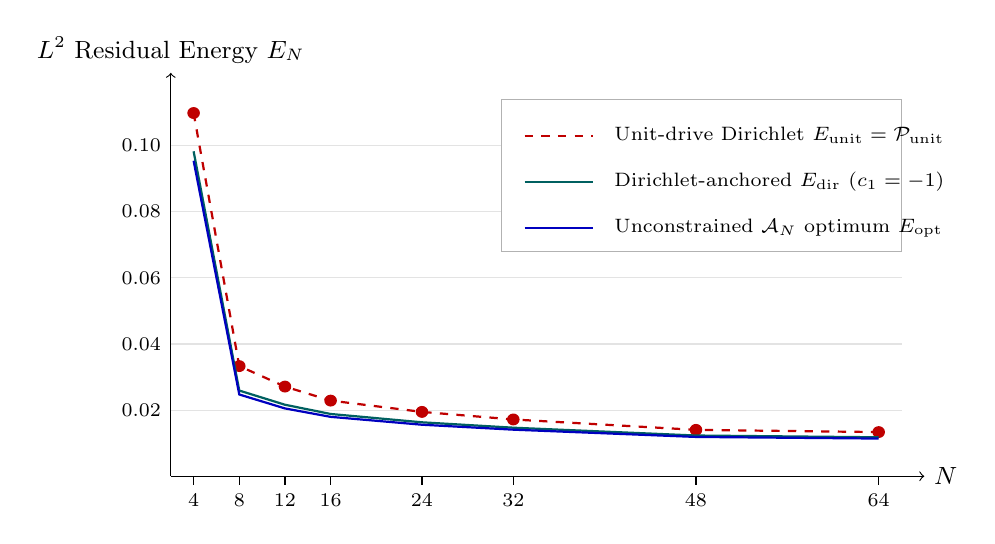
\begin{tikzpicture}[xscale=0.145,yscale=42]
  % Axes
  \draw[->] (2,0) -- (68,0) node[right,font=\small] {$N$};
  \draw[->] (2,0) -- (2,0.122) node[above,font=\small] {$L^2$ Residual Energy $E_N$};
  % Grid & Ticks
  \foreach \y in {0.02,0.04,0.06,0.08,0.10} {
    \draw[gray!22] (2,\y) -- (66,\y);
    \node[left,font=\scriptsize] at (2,\y) {\y};
  }
  \foreach \x in {4,8,12,16,24,32,48,64} {
    \draw (\x,0) -- (\x,-0.0025) node[below,font=\scriptsize] {\x};
  }
  % E_unit = P_unit (red dashed)
  \draw[red!75!black,thick,dashed]
    (4,0.109836) -- (8,0.033308) -- (12,0.027108) -- (16,0.022875) --
    (24,0.019456) -- (32,0.017171) -- (48,0.014025) -- (64,0.013351);
  \foreach \p in {(4,0.109836),(8,0.033308),(12,0.027108),(16,0.022875),(24,0.019456),(32,0.017171),(48,0.014025),(64,0.013351)} {
    \fill[red!75!black] \p circle[x radius=0.55,y radius=0.0018];
  }
  % E_dir (teal dotted-solid)
  \draw[teal!75!black,thick]
    (4,0.098247) -- (8,0.025908) -- (12,0.021616) -- (16,0.018833) --
    (24,0.016312) -- (32,0.014681) -- (48,0.012317) -- (64,0.011787);
  % E_opt (blue solid)
  \draw[blue!75!black,thick]
    (4,0.095394) -- (8,0.024715) -- (12,0.020509) -- (16,0.017959) --
    (24,0.015578) -- (32,0.014085) -- (48,0.011893) -- (64,0.011392);
  % Legend box
  \draw[fill=white,draw=gray!60] (31,0.068) rectangle (66,0.114);
  \draw[red!75!black,thick,dashed] (33,0.103) -- (39,0.103);
  \node[right,font=\scriptsize] at (40,0.103) {Unit-drive Dirichlet $E_{\mathrm{unit}} = \mathcal{P}_{\mathrm{unit}}$};
  \draw[teal!75!black,thick] (33,0.089) -- (39,0.089);
  \node[right,font=\scriptsize] at (40,0.089) {Dirichlet-anchored $E_{\mathrm{dir}}$ ($c_1 = -1$)};
  \draw[blue!75!black,thick] (33,0.075) -- (39,0.075);
  \node[right,font=\scriptsize] at (40,0.075) {Unconstrained $\mathcal{A}_N$ optimum $E_{\mathrm{opt}}$};
\end{tikzpicture}
\caption{Comparison of finite-$N$ Nyman--Beurling $L^2$ residuals under unconstrained $\mathcal{A}_N$ optimization, Dirichlet anchoring ($c_1 = -1$), and simultaneous unit-drive Dirichlet normalization ($E_{\mathrm{unit}} = \mathcal{P}_{\mathrm{unit}}$).}
\label{fig:dirichlet_energies}
\end{figure}

Table~\ref{tab:dirichlet_lab} and Figure~\ref{fig:dirichlet_energies} illustrate two structural phenomena across $N \le 64$: (a) unconstrained $c_{1,\mathrm{opt}}^{(N)}$ approaches $-1$ from above after $N=8$ ($-0.9539$ at $N=8$ to $-0.9725$ at $N=64$), incurring only a $3.5\%$ penalty between $E_{\mathrm{dir}}^{(64)} = 0.011787$ and $E_{\mathrm{opt}}^{(64)} = 0.011392$; and (b) enforcing the additional unit-drive hyperplane $\pi L_{\mathrm{cot}} = 1$ lowers the ratio $E_{\mathrm{unit}}^{(N)}/E_{\mathrm{opt}}^{(N)}$ monotonically from $1.3477$ ($N=8$) to $1.1719$ ($N=64$). Across every horizon and all three families, the discrete 2D telescoping formula~\eqref{eq:form_tel} agrees with $\alpha^\top P \alpha$ to $< 2.7 \times 10^{-86}$ while maintaining $D_0 = 2$ and $D_1 = 0$ to $< 1.5 \times 10^{-85}$. No unconditional conclusion about the asymptotic decay of $\mathcal{P}_N$ as $N \to \infty$ is claimed (\texttt{NO\_RH\_PROOF = TRUE}).

\begin{thebibliography}{9}
\bibitem{BaezDuarte2003}
L.~B\'aez-Duarte, A strengthening of the Nyman--Beurling criterion for the Riemann hypothesis, \emph{Rend.\ Mat.\ Acc.\ Lincei} \textbf{14} (2003), 5--11.

\bibitem{Vasyunin1995}
V.~I.~Vasyunin, On a biorthogonal system associated with the Riemann hypothesis, \emph{Algebra i Analiz} \textbf{7} (1995), 118--135.

\bibitem{PaperJ}
Q.~Munawer, Pure 4-Point Plaque Reduction, Anchor-Drive Cancellation, and the Diagonal/Off-Diagonal Asymptotic Frontier on $\mathcal{A}_N$, Zenodo DOI \href{https://doi.org/10.5281/zenodo.24330500}{10.5281/zenodo.24330500} (2026).

\bibitem{RiemannBlueprint}
Q.~Munawer, \emph{RiemannBlueprint: Verified Modular Lean~4.35.0 Formalizations} ($53$ Self-Contained Modular Units, \texttt{NO\_RH\_PROOF = TRUE}), Zenodo Master Archive Hub~07, DOI \href{https://doi.org/10.5281/zenodo.24329861}{10.5281/zenodo.24329861} (2026).
\end{thebibliography}

\end{document}
